% ============================================================
% 第 3 章  伪微分算子的量子化（续）
% ch03b：原书 p.180–192（PDF 181–193），含 §3.4–§3.6 与本章回顾
% ============================================================

% [块界：本块自原书 p.180 顶部起，首行是定理 3.3.6（驻相渐近展开）证明的后半段。该定理的陈述与原书 p.179 的正文并入上一块 ch03a，本块不重复陈述，只从证明开头接着译。]

% [原文 p.180]
\begin{proof}[定理 3.3.6 的证明]
设 \(x_0=0\) 且 \(\varphi(0)=0\)。由莫尔斯引理，存在局部坐标变换 \(\{y^i(x)\}\)，使得
\[
  \varphi(x)=\frac{1}{2}\left(y_1^2+\cdots+y_r^2-y_{r+1}^2-\cdots-y_n^2\right).
\]
这里 \(r=\sgn\partial^2\varphi(0)\)。设 \(\chi\) 是在 \(x_0=0\) 附近等于 \(1\) 的截断函数。则
\begin{align*}
  \int_{\R^n}e^{\frac{i}{\hbar}\varphi(x)}a(x)\,dx
  &=\int_{\R^n}e^{\frac{i}{\hbar}\varphi(x)}\chi(x)a(x)\,dx+O(\hbar^\infty)\\
  &=\int_{\R^n}e^{\frac{i}{2\hbar}A(y)}u(y)\,dy+O(\hbar^\infty)
\end{align*}
其中
\[
  u(y)=\chi(x(y))a(x(y))\left|\det\left(\frac{\partial x}{\partial y}\right)\right|,
  \qquad
  A=\begin{pmatrix}I_r&\\ &-I_{n-r}\end{pmatrix}.
\]
应用命题 3.3.5，我们得到
\[
  \int_{\R^n}e^{\frac{i}{\hbar}\varphi(x)}a(x)\,dx
  \sim (2\pi\hbar)^{\frac{n}{2}}\frac{e^{\frac{i\pi}{4}\sgn A}}{\sqrt{|\det A|}}
  \sum_{k=0}^{\infty}\frac{\hbar^k}{k!}\left(\frac{A^{-1}(D)}{2i}\right)^k u(0).
\]
注意 \(\sgn A=\sgn\partial^2\varphi\)，并且
\[
  \det\partial_{x_i}\partial_{x_j}\varphi(x_0)
  =\left(\det\left(\frac{\partial y}{\partial x}\right)(x_0)\right)^2\det A,
\]
并且由上式得到
\[
  \left|\det\left(\frac{\partial x}{\partial y}\right)(x_0)\right|
  =\frac{1}{\sqrt{\left|\det\partial^2\varphi(x_0)\right|}}.
\]
由此得到首项
\[
  A_0=\frac{e^{\frac{i}{4}\pi\sgn\partial^2\varphi(x_0)}}{\sqrt{\left|\det\partial^2\varphi(x_0)\right|}}.
\]
\end{proof}

\begin{example}{3.3.7}
设 \(A\) 是实对称非奇异矩阵，\(\phi(x)\in C_c^\infty(\R^n)\)。我们已经看到
\[
  e^{\frac{i\hbar}{2}A(D_x)}\phi(x)
  =\frac{e^{\frac{i\pi}{4}\sgn A}}{(2\pi\hbar)^{\frac{n}{2}}\sqrt{|\det A|}}
  \int_{\R^n}e^{-\frac{i}{2\hbar}A^{-1}(y)}\phi(x+y)\,dy.
\]
另一方面，应用命题 3.3.5 可得
\[
  \int_{\R^n}e^{-\frac{i}{2\hbar}A^{-1}(y)}\phi(x+y)\,dy
  \sim (2\pi\hbar)^{\frac{n}{2}}\frac{e^{-\frac{i\pi}{4}\sgn A}}{\sqrt{|\det A^{-1}|}}
  \sum_{k=0}^{\infty}\frac{\hbar^k}{k!}\left(\frac{i\hbar A(D_x)}{2}\right)^k\phi(x).
\]
于是
\[
  e^{\frac{i\hbar}{2}A(D_x)}\phi(x)
  \sim\sum_{k=0}^{\infty}\frac{\hbar^k}{k!}\left(\frac{i\hbar A(D_x)}{2}\right)^k\phi(x).
\]
这个渐近公式为符号 \(e^{\frac{i\hbar}{2}A(D_x)}\) 提供了依据。
\end{example}

\takeaway{本节定义振荡积分 \(\int e^{\frac{i}{\hbar}\varphi}a\)：无驻点时它 \(O(\hbar^\infty)\)；在非退化临界点附近用莫尔斯引理把相位化为二次型，得到驻定相位的首项公式，其系数含 \(\sqrt{|\det\partial^2\varphi|^{-1}}\) 与 \(e^{\frac{i}{4}\pi\sgn\partial^2\varphi}\) 的相位修正。后文的连接公式与渐近展开都由此而来。}

\section{复合公式}

\subsection{外尔量子化与 Moyal 乘积}

给定来自符号 \(a,b\in S(\R^{2n})\) 的两个量子化算子，例如外尔量子化下的 \(a^W\) 与 \(b^W\)，它们的复合 \(a^W\circ b^W\) 仍是量子化算子 \((a\star b)^W\)，对应的符号为 \(a\star b\)
\[
  a^W\circ b^W=(a\star b)^W.
\]
% [原文 p.181]
这里 \(a\star b\) 称为符号 \(a\) 与 \(b\) 的\emph{Moyal 乘积}。

为看清它的样子，取 \(\varphi\in S(\R^n)\)，用核函数计算
\[
  a^W\circ b^W(\varphi)(x)
  =\int_{\R^n}\int_{\R^n}K_a^W(x,z)K_b^W(z,y)\varphi(y)\,dy\,dz.
\]
于是 \(a^W\circ b^W\) 的核函数为
\begin{align*}
  &\int_{\R^n}K_a^W(x,z)K_b^W(z,y)\,dz\\
  &=\frac{1}{(2\pi\hbar)^{2n}}\int_{(\R^n)^3}
    e^{\frac{i}{\hbar}\langle x-z,\eta_1\rangle}
    e^{\frac{i}{\hbar}\langle z-y,\eta_2\rangle}\\
  &\qquad\times
    a\left(\frac{x+z}{2},\eta_1\right)b\left(\frac{z+y}{2},\eta_2\right)
    \,d\eta_1d\eta_2dz\\
  &=\frac{1}{(2\pi\hbar)^{2n}}\int_{(\R^n)^4}
    e^{\frac{i}{\hbar}\langle x-z_2,\eta_1\rangle}
    e^{\frac{i}{\hbar}\langle z_1-y,\eta_2\rangle}\\
  &\qquad\times\delta(z_2-z_1)
    a\left(\frac{x+z_1}{2},\eta_1\right)b\left(\frac{z_2+y}{2},\eta_2\right)
    \,dz_1dz_2d\eta_1d\eta_2\\
  &=\frac{1}{(2\pi\hbar)^{3n}}\int_{(\R^n)^5}
    e^{\frac{i}{\hbar}\langle x-z_2,\eta_1\rangle}
    e^{\frac{i}{\hbar}\langle z_1-y,\eta_2\rangle}
    e^{\frac{i}{\hbar}\langle z_2-z_1,\xi\rangle}\\
  &\qquad\times
    a\left(\frac{x+z_1}{2},\eta_1\right)b\left(\frac{z_2+y}{2},\eta_2\right)
    \,d\xi dz_1dz_2d\eta_1d\eta_2\\
  &=\frac{1}{(2\pi\hbar)^{3n}}\int_{(\R^n)^5}
    e^{\frac{i}{\hbar}\langle x-z_2,\eta_1-\xi\rangle}
    e^{\frac{i}{\hbar}\langle z_1-y,\eta_2-\xi\rangle}
    e^{\frac{i}{\hbar}\langle x-y,\xi\rangle}\\
  &\qquad\times
    a\left(\frac{x+y}{2}+\frac{z_1-y}{2},\xi+\eta_1-\xi\right)\\
  &\qquad\times
    b\left(\frac{x+y}{2}+\frac{z_2-x}{2},\xi+\eta_2-\xi\right)\\
  &\qquad\times d\xi dz_1dz_2d\eta_1d\eta_2\\
  &=\frac{2^{2n}}{(2\pi\hbar)^{3n}}\int_{(\R^n)^5}
    e^{\frac{i}{\hbar}\langle x-y,\xi\rangle}
    e^{\frac{2i}{\hbar}\left(\langle z_1,\eta_2\rangle-\langle z_2,\eta_1\rangle\right)}\\
  &\qquad\times
    a\left(\frac{x+y}{2}+z_1,\xi+\eta_1\right)\\
  &\qquad\times
    b\left(\frac{x+y}{2}+z_2,\xi+\eta_2\right)\\
  &\qquad\times dz_1dz_2d\eta_1d\eta_2d\xi.
\end{align*}
这里最后一步我们作了变量替换。

与外尔量子化的核公式
\[
  K_{a\star b}^W=\frac{1}{(2\pi\hbar)^{n}}\int_{\R^n}
  e^{\frac{i}{\hbar}\langle x-y,\xi\rangle}(a\star b)\left(\frac{x+y}{2},\xi\right)d\xi
\]
比较，我们得到 Moyal 乘积的如下积分公式
\[
  \begin{aligned}
    (a\star b)(x,\xi)
    &=\frac{1}{(\pi\hbar)^{2n}}\int_{(\R^n)^4}
      e^{\frac{2i}{\hbar}\left(\langle z_1,\eta_2\rangle-\langle z_2,\eta_1\rangle\right)}\\
    &\qquad\qquad\times
      a(x+z_1,\xi+\eta_1)b(x+z_2,\xi+\eta_2)\,dz_1dz_2d\eta_1d\eta_2.
  \end{aligned}
\]
我们还可以借助微分算子来表示这个公式，利用
\begin{align*}
  &a(x+z_1,\xi+\eta_1)b(x+z_2,\xi+\eta_2)\\
  &\quad=a(x_1+z_1,\xi_1+\eta_1)b(x_2+z_2,\xi_2+\eta_2)\Big|_{\substack{x_1=x_2=x\\ \xi_1=\xi_2=\xi}}\\
  &\quad=e^{\frac{i}{\hbar}\langle z_1,D_{x_1}^\hbar\rangle}
    e^{\frac{i}{\hbar}\langle\eta_1,D_{\xi_1}^\hbar\rangle}
    e^{\frac{i}{\hbar}\langle z_2,D_{x_2}^\hbar\rangle}
    e^{\frac{i}{\hbar}\langle\eta_2,D_{\xi_2}^\hbar\rangle}
    a(x_1,\xi_1)b(x_2,\xi_2)\Big|_{\substack{x_1=x_2=x\\ \xi_1=\xi_2=\xi}}.
\end{align*}
形式上，
\begin{align*}
  &\frac{1}{(\pi\hbar)^{2n}}\int_{(\R^n)^4}
    e^{\frac{2i}{\hbar}\left(\langle z_1,\eta_2\rangle-\langle z_2,\eta_1\rangle\right)}
    e^{\frac{i}{\hbar}\left(\langle z_1,D_{x_1}^\hbar\rangle
      +\langle\eta_1,D_{\xi_1}^\hbar\rangle
      +\langle z_2,D_{x_2}^\hbar\rangle
      +\langle\eta_2,D_{\xi_2}^\hbar\rangle\right)}
    dz_1dz_2d\eta_1d\eta_2\\
  &=\frac{1}{(2\pi\hbar)^{2n}}\int_{(\R^n)^4}
    e^{\frac{i}{\hbar}\left\langle z_1,\eta_2+\frac{1}{2}D_{x_1}^\hbar\right\rangle}
    e^{-\frac{i}{\hbar}\left\langle z_2,\eta_1-\frac{1}{2}D_{x_2}^\hbar\right\rangle}
    e^{\frac{i}{\hbar}\left(\langle\eta_1,D_{\xi_1}^\hbar\rangle
      +\langle\eta_2,D_{\xi_2}^\hbar\rangle\right)}
    dz_1dz_2d\eta_1d\eta_2\\
  &=\int_{(\R^n)^2}
    e^{\frac{i}{\hbar}\left(\langle\eta_1,D_{\xi_1}^\hbar\rangle
      +\langle\eta_2,D_{\xi_2}^\hbar\rangle\right)}
    \delta\left(\eta_2+\frac{1}{2}D_{x_1}^\hbar\right)
    \delta\left(\eta_1-\frac{1}{2}D_{x_2}^\hbar\right)d\eta_1d\eta_2\\
  &=e^{\frac{i}{2\hbar}\left(\langle D_{\xi_1}^\hbar,D_{x_2}^\hbar\rangle
    -\langle D_{x_1}^\hbar,D_{\xi_2}^\hbar\rangle\right)}\\
  &=e^{\frac{i\hbar}{2}\left(\langle D_{\xi_1},D_{x_2}\rangle
    -\langle D_{x_1},D_{\xi_2}\rangle\right)}
\end{align*}

% [原文 p.182]
它是二次指数的量子化。上面的形式计算可以借助缓增分布意义下的傅里叶变换严格化。细节留给读者（参见 Zworski 的书）。

于是我们得到施瓦茨符号的 Moyal 乘积的如下复合公式。

\begin{proposition}{3.4.1}
设 \(a,b\in S(\R^{2n})\)。则 \(a^W\circ b^W=(a\star b)^W\)，其中
\begin{align*}
  (a\star b)(x,\xi)
  &=\frac{1}{(\pi\hbar)^{2n}}\int_{(\R^n)^4}
    e^{\frac{2i}{\hbar}\left(\langle z_1,\eta_2\rangle-\langle z_2,\eta_1\rangle\right)}\\
  &\qquad\qquad\times
    a(x+z_1,\xi+\eta_1)b(x+z_2,\xi+\eta_2)\,dz_1dz_2d\eta_1d\eta_2\\
  &=e^{\frac{i\hbar}{2}\left(\langle D_{\xi_1},D_{x_2}\rangle-\langle D_{x_1},D_{\xi_2}\rangle\right)}\\
  &\qquad\qquad\times
    a(x_1,\xi_1)b(x_2,\xi_2)\Big|_{\substack{x_1=x_2=x\\ \xi_1=\xi_2=\xi}}.
\end{align*}
\end{proposition}

应用驻相法可得 \(\hbar\)-渐近展开
\[
  (a\star b)(x,\xi)
  \sim\sum_{k=0}^{\infty}\frac{(i\hbar)^k}{k!}
  \left[\frac{1}{2}\langle D_{\xi_1},D_{x_2}\rangle
    -\frac{1}{2}\langle D_{x_1},D_{\xi_2}\rangle\right]^k
  a(x_1,\xi_1)b(x_2,\xi_2)\Big|_{\substack{x_1=x_2=x\\ \xi_1=\xi_2=\xi}}.
\]
特别地，
\[
  a\star b\sim 0
  \qquad\text{若}\qquad \supp(a)\cap\supp(b)=\varnothing.
\]

\subsection{科恩–尼伦伯格量子化}

现在考虑标准量子化（科恩–尼伦伯格量子化，Kohn–Nirenberg quantization）的复合公式。核函数为
\[
  K_a(x,y)=\frac{1}{(2\pi\hbar)^{n}}\int_{\R^n}
  e^{\frac{i}{\hbar}\langle x-y,\xi\rangle}a(x,\xi)\,d\xi.
\]
我们用同样的方法计算
\[
  a^{KN}\circ b^{KN}=(a\star_{KN}b)^{KN}
\]
其中 \(\star_{KN}\) 表示标准量子化下符号的复合。

\(a^{KN}\circ b^{KN}\) 的核函数为
\begin{align*}
  &\int_{\R^n}K_a(x,z)K_b(z,y)\,dz\\
  &=\frac{1}{(2\pi\hbar)^{2n}}\int_{(\R^n)^3}
    e^{\frac{i}{\hbar}\langle x-z,\eta\rangle+\frac{i}{\hbar}\langle z-y,\xi\rangle}
    a(x,\eta)b(z,\xi)\,d\eta d\xi dz\\
  &=\frac{1}{(2\pi\hbar)^{2n}}\int_{(\R^n)^3}
    e^{\frac{i}{\hbar}\langle x-y,\xi\rangle}
    e^{\frac{i}{\hbar}\langle x-z,\eta-\xi\rangle}
    a(x,\xi+\eta-\xi)b(x+z-x,\xi)\,d\eta d\xi dz\\
  &=\frac{1}{(2\pi\hbar)^{2n}}\int_{(\R^n)^3}
    e^{\frac{i}{\hbar}\langle x-y,\xi\rangle}
    e^{-\frac{i}{\hbar}\langle z,\eta\rangle}
    a(x,\xi+\eta)b(x+z,\xi)\,d\eta dz d\xi.
\end{align*}
将这与标准量子化的核函数
\[
  K_{a\star_{KN}b}(x,\xi)
  =\frac{1}{(2\pi\hbar)^{n}}\int_{\R^n}
  e^{-\frac{i}{\hbar}\langle x-y,\xi\rangle}(a\star_{KN}b)(x,\xi)\,d\xi
\]
比较，我们得到如下积分公式
\[
  (a\star_{KN}b)(x,\xi)
  =\frac{1}{(2\pi\hbar)^{n}}\int_{(\R^n)^2}
  e^{-\frac{i}{\hbar}\langle z,\eta\rangle}a(x,\xi+\eta)b(x+z,\xi)\,dz d\eta.
\]

% [原文 p.183]
这同样可以用二次指数表示
\[
  a(x,\xi+\eta)b(x+z,\xi)
  =e^{\frac{i}{\hbar}\langle\eta,D_\xi^\hbar\rangle}
  e^{\frac{i}{\hbar}\langle z,D_x^\hbar\rangle}
  a(\tilde x,\tilde\xi)b(\tilde x,\tilde\xi)
  \Big|_{\substack{\tilde\xi=\xi\\ \tilde x=x}}.
\]
我们作类似的形式演算
\begin{align*}
  &\frac{1}{(2\pi\hbar)^{n}}\int_{(\R^n)^2}
    e^{-\frac{i}{\hbar}\langle x,\eta\rangle}
    e^{\frac{i}{\hbar}\langle\eta,D_\xi^\hbar\rangle}
    e^{\frac{i}{\hbar}\langle z,D_x^\hbar\rangle}
    dz\,d\eta\\
  &=\int_{\R^n}
    e^{\frac{i}{\hbar}\langle\eta,D_\xi^\hbar\rangle}
    \delta(\eta-D_x^\hbar)\,d\eta\\
  &=e^{\frac{i}{\hbar}\langle D_\xi^\hbar,D_x^\hbar\rangle}\\
  &=e^{i\hbar\langle D_\xi,D_x\rangle}.
\end{align*}
这些计算在傅里叶变换下恰当进行，就给出标准量子化的复合公式。

\begin{proposition}{3.4.2}
  设 \(a,b\in S(\R^{2n})\)。则 \(a^{KN}\circ b^{KN}=(a\star_{KN}b)^{KN}\)，其中
  \begin{align*}
    &(a\star_{KN}b)(x,\xi)\\
    &=\frac{1}{(2\pi\hbar)^{n}}\int_{(\R^n)^2}
      e^{-\frac{i}{\hbar}\langle z,\eta\rangle}
      a(x,\xi+\eta)b(x+z,\xi)\,dz\,d\eta\\
    &=e^{i\hbar\langle D_\xi,D_x\rangle}
      a(\tilde x,\tilde\xi)b(\tilde x,\tilde\xi)
      \Big|_{\substack{\tilde\xi=\xi\\ \tilde x=x}}.
  \end{align*}
\end{proposition}

应用驻相法可得 \(\hbar\)-渐近展开
\[
  (a\star_{KN}b)(x,\xi)
  \sim\sum_{k=0}^{\infty}\frac{(i\hbar)^k}{k!}
  \langle D_\xi,D_x\rangle^k
  a(\tilde x,\tilde\xi)b(\tilde x,\tilde\xi)
  \Big|_{\substack{\tilde\xi=\xi\\ \tilde x=x}}.
\]

\takeaway{本节把量子化的复合写成象征的乘法。外尔量子化与标准量子化各自给出一个星乘积：前者是 Moyal 乘积，其核函数由外尔核的卷积算出；后者是科恩–尼伦伯格乘积。两个乘积都有积分表示，也都能借驻相法写成微分算子的指数形式，从而得到 $\hbar$ 的渐近展开式的首项。}

\section{带阶函数的象征类}

\noindent\textbf{记号}：\(\langle x\rangle=(1+|x|^2)^{\frac12}\)，\(x\in\R^d\)。

\subsection{阶函数与象征类}

\begin{definition}{3.5.1}
  函数 \(m:\R^d\to\R_+\) 称为\emph{阶函数}（order function），若存在常数 \(C\) 与 \(N\)，使得
  \[
    m(x)\le C\langle x-y\rangle^{N}m(y),\qquad \forall x,y\in\R^d.
  \]
\end{definition}

\begin{proposition}{3.5.2}
  若 \(m_1,m_2\) 是阶函数，则 \(m_1+m_2\) 与 \(m_1^{a}m_2^{b}\) 对任意 \(a,b\in\R\) 都是阶函数。
\end{proposition}

\begin{example}{3.5.3}
  下列函数是常用的阶函数
  \begin{itemize}[leftmargin=2em,itemsep=1pt]
    \item \(m(x)=\langle x\rangle\) 是 \(\R^d\) 上的阶函数。
    % [原文 p.184]
    \item 考虑带坐标 \((x,\xi)\) 的 \(\R^{2n}\)。则
    \[
      m(x,\xi)=\langle x\rangle^{a}\langle\xi\rangle^{b}
    \]
    对任意 \(a,b\in\R\) 都是阶函数。
  \end{itemize}
\end{example}

\begin{definition}{3.5.4}
  设 \(m\) 是 \(\R^d\) 上的阶函数。定义在 \(\R^d\times(0,h_0]\) 上的光滑函数 \(\varphi(x,\hbar)\)（其中某个 \(h_0>0\)）称为
  \begin{itemize}[leftmargin=2em,itemsep=1pt]
    \item 属于 \(S(m)\)，若对任意多指标 \(\alpha\)，
    \[
      \partial^\alpha\varphi=O(m)\qquad
      (\text{在 }\R^d\times(0,h_0]\text{ 上一致成立})
    \]
    \item 属于 \(S_\delta(m)\)，若对任意多指标 \(\alpha\)，
    \[
      \partial^\alpha\varphi=O(\hbar^{-\delta|\alpha|}m)\qquad
      (\text{在 }\R^d\times(0,h_0]\text{ 上一致成立})
    \]
    \item 属于 \(S_\delta^{k}(m)\)（\(0\le\delta\le\frac12\)），若对任意多指标 \(\alpha\)，
    \[
      \partial^\alpha\varphi=O(\hbar^{-\delta|\alpha|-k}m)\qquad
      (\text{在 }\R^d\times(0,h_0]\text{ 上一致成立})
    \]
  \end{itemize}
  我们还会写
  \[
    S_\delta^{-\infty}(m):=\bigcap_{N=0}^{\infty}S_\delta^{-N}(m).
  \]
\end{definition}

\subsubsection*{量子化}

现在我们考虑相位空间 \(\R^{2n}\)，并选定一个阶函数 \(m\)。显然
\[
  S(\R^{2n})\subset S(m)\ \text{或}\ S_\delta(m).
\]
我们可以把量子化从施瓦茨函数自然延拓到这些象征类。

\begin{proposition}{3.5.5}
  设 \(a\in S_\delta(m)\)。则外尔量子化
  \[
    \left(a^Wu\right)(x)
    =\frac{1}{(2\pi\hbar)^{n}}\int_{\R^n}\int_{\R^n}
    e^{\frac{i}{\hbar}\langle x-y,\xi\rangle}
    a\left(\frac{x+y}{2},\xi\right)u(y)\,dy\,d\xi
  \]
  定义了连续线性映射
  \[
    a^W:S(\R^n)\longrightarrow S(\R^n)
    \qquad\text{以及}\qquad
    a^W:S'(\R^n)\longrightarrow S'(\R^n).
  \]
  这里 \(\hbar>0\) 固定。
\end{proposition}

\begin{proof}
  考虑微分算子
  \begin{align*}
    L_1&=\frac{1-\langle\xi,D_y^\hbar\rangle}{1+|\xi|^2},
    &L_1^*&=\frac{1+\langle\xi,D_y^\hbar\rangle}{1+|\xi|^2},\\
    L_2&=\frac{1+\langle x-y,D_\xi^\hbar\rangle}{1+|x-y|^2},
    &L_2^*&=\frac{1-\langle x-y,D_\xi^\hbar\rangle}{1+|x-y|^2}
  \end{align*}
% [原文 p.185]
  它们满足
  \[
    L_1e^{\frac{i}{\hbar}\langle x-y,\xi\rangle}
    =L_2e^{\frac{i}{\hbar}\langle x-y,\xi\rangle}
    =e^{\frac{i}{\hbar}\langle x-y,\xi\rangle}.
  \]
  设 \(m(z)\le C\langle z-w\rangle^{N}m(w)\)，其中 \(z=(x,\xi)\)。则
  \begin{align*}
    (a^Wu)(x)
    &=\frac{1}{(2\pi\hbar)^{n}}\int_{\R^n}\int_{\R^n}
      \left(L_1^{k}L_2^{l}e^{\frac{i}{\hbar}\langle x-y,\xi\rangle}\right)
      a\left(\frac{x+y}{2},\xi\right)u(y)\,dy\,d\xi\\
    &=\frac{1}{(2\pi\hbar)^{n}}\int_{\R^n}\int_{\R^n}
      e^{\frac{i}{\hbar}\langle x-y,\xi\rangle}
      (L_2^{*})^{l}(L_1^{*})^{k}
      \left(a\left(\frac{x+y}{2},\xi\right)u(y)\right)dy\,d\xi\\
    &=\frac{1}{(2\pi\hbar)^{n}}\int_{\R^n}\int_{\R^n}
      e^{\frac{i}{\hbar}\langle x-y,\xi\rangle}
      \langle x-y\rangle^{-2l}
      \left(1-\langle x-y,D_\xi^\hbar\rangle\right)^{l}\\
    &\qquad\times\left(\langle\xi\rangle^{-2k}
      \left(1+\langle\xi,D_y^\hbar\rangle\right)^{k}
      \left(a\left(\frac{x+y}{2},\xi\right)u(y)\right)\right)dy\,d\xi.
  \end{align*}
  由于 \(a\in S_\delta(m)\)，
  \begin{align*}
    &\left|D_\xi^\alpha D_y^\beta a\left(\frac{x+y}{2},\xi\right)\right|\\
    &\qquad\le C_{\alpha\beta}\hbar^{-\delta(|\alpha|+|\beta|)}
      m\left(\frac{x+y}{2},\xi\right)\\
    &\qquad\le C_{\alpha\beta}\hbar^{-\delta(|\alpha|+|\beta|)}
      \left\langle\frac{x-y}{2}\right\rangle^{N}
      \langle\xi\rangle^{N}m(y,0).
  \end{align*}
  由于 \(u\) 是施瓦茨函数，取 \(k,l\) 充分大即得
  \[
    \left|(a^Wu)(x)\right|\le C'
  \]
  其中 \(C'\) 是某个常数。于是
  \[
    a^Wu\in L^\infty(\R^n).
  \]
  其次注意
  \begin{align*}
    x^\alpha(a^Wu)(x)
    &=\frac{1}{(2\pi\hbar)^{n}}\int_{\R^n}\int_{\R^n}
      \left(\left(D_\xi^\hbar+y\right)^{\alpha}
      e^{\frac{i}{\hbar}\langle x-y,\xi\rangle}\right)
      a\left(\frac{x+y}{2},\xi\right)u(y)\,dy\,d\xi\\
    &=\frac{1}{(2\pi\hbar)^{n}}\int_{\R^n}\int_{\R^n}
      e^{\frac{i}{\hbar}\langle x-y,\xi\rangle}
      \left(-D_\xi^\hbar+y\right)^{\alpha}
      \left(a\left(\frac{x+y}{2},\xi\right)u(y)\right)dy\,d\xi.
  \end{align*}
  由与上面相同的论证，
  \[
    x^{\alpha}a^Wu\in L^\infty(\R^n),\qquad \forall\ \text{多指标 }\alpha.
  \]
  类似的论证还给出
  \[
    x^{\alpha}\partial^{\beta}(a^Wu),\qquad \forall\ \text{多指标 }\alpha,\beta,
  \]
  从而 \(a^Wu\in S(\R^n)\)。

  上面的论证同时表明：若 \(u_j\) 的半范数趋于 \(0\)，则 \(a^Wu_j\) 的半范数也趋于 \(0\)。这说明 \(a^W:S(\R^n)\to S(\R^n)\) 连续。对 \(a^W:S'(\R^n)\to S'(\R^n)\) 的结论由对偶性得到，依据是
  \[
    \langle a^W(x,D_x^\hbar)u,v\rangle
    =\langle u,a^W(x,-D_x^\hbar)v\rangle.
  \]
\end{proof}

% [原文 p.186]
\subsection{渐近展开}

\begin{definition}{3.5.6}
  设 \(a_j\in S_\delta(m)\)。我们称 \(a\in S_\delta(m)\) 渐近于
  \(\sum_{j=0}^{\infty}\hbar^{j}a_j\)，并记
  \[
    a\sim\sum_{j=0}^{\infty}\hbar^{j}a_j,
  \]
  若对任意正整数 \(N\) 都有
  \[
    a-\sum_{j=0}^{N-1}\hbar^{j}a_j\in S_\delta^{-N}(m).
  \]
  首项 \(a_0\) 称为 \(a\) 的\emph{主象征}（principal symbol）。
\end{definition}

\begin{theorem}{3.5.7}
  （博雷尔引理）对任意序列 \(a_j\in S_\delta(m)\)，\(j=0,1,\cdots\)，存在 \(a\in S_\delta(m)\) 使得
  \[
    a\sim\sum_{j=0}^{\infty}\hbar^{j}a_j
    \qquad\text{在 }S_\delta(m)\text{ 中}.
  \]
  对另一个满足 \(\tilde a\sim\sum_{j=0}^{\infty}\hbar^{j}a_j\) 的 \(\tilde a\in S_\delta(m)\)，我们有 \(\tilde a-a\in S_\delta^{-\infty}(m)\)。
\end{theorem}

\begin{proof}
  设 \(0<\hbar\le1\)。选取光滑截断函数 \(\chi\)，使得
  \[
    \begin{cases}
      \chi(t)=1, & 0\le t\le1,\\
      0\le\chi(t)\le1, & 1\le t\le2,\\
      \chi(t)=0, & t\ge2,\\
      \chi(t)\le\dfrac{2}{t}, & t>0.
    \end{cases}
  \]
  \begin{center}
    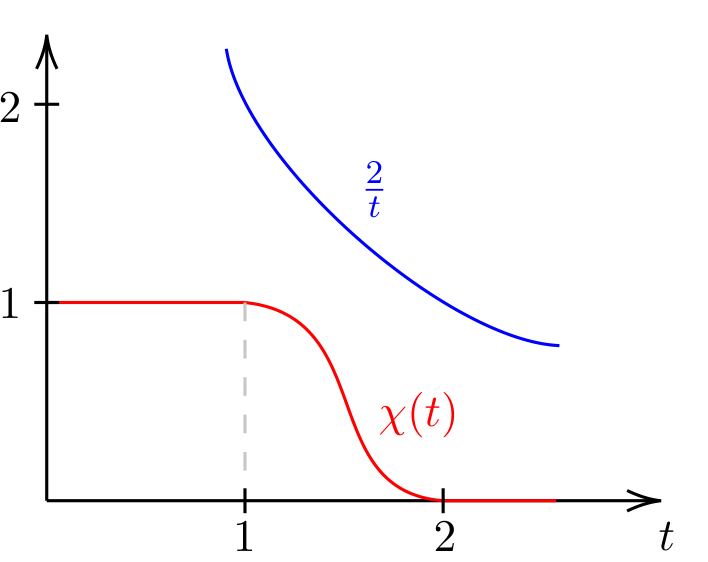
\includegraphics[width=0.42\textwidth]{figures/fig_p187_a.png}
  \end{center}
  % [图：原书 p.186，图内文字照原样保留]
  考虑
  \[
    a=\sum_{j=0}^{\infty}\hbar^{j}\chi(\lambda_j\hbar)a_j,
  \]
  其中序列 \(\lambda_j\nearrow+\infty\) 待选。由于 \(\lambda_j\to\infty\)，对每个 \(\hbar>0\) 求和式中只有有限多项非零。

  现在说明如何选取这样的 \(\{\lambda_j\}\)。对每个多指标 \(\alpha\)，由于 \(a_j\in S_\delta(m)\)，
  \[
    \hbar^{j}\chi(\lambda_j\hbar)\left|\partial^{\alpha}a_j\right|
    \le C_{j,\alpha}\hbar^{j-\delta|\alpha|}
    \chi(\lambda_j\hbar)m
    \le C_{j,\alpha}\hbar^{j-\delta|\alpha|}
    \frac{2}{\lambda_j\hbar}m
    =2C_{j,\alpha}\frac{\hbar^{j-1-\delta|\alpha|}}{\lambda_j}m.
  \]

% [原文 p.187]
  我们选取递增的 \(\lambda_j\)，使得
  \[
    \frac{2C_{j,\alpha}}{\lambda_j}\le2^{-j},
    \qquad \text{对所有 }|\alpha|\le j.
  \]
  于是对任意 \(|\alpha|\le j\) 有
  \[
    \hbar^{j}\chi(\lambda_j\hbar)\left|\partial^\alpha a_j\right|
    \le\hbar^{j-1-\delta|\alpha|}2^{-j}m.
  \]
  下面说明我们构造的函数 \(a\) 具有所期望的渐近展开。
  \begin{align*}
    a-\sum_{j=0}^{N-1}\hbar^{j}a_j
    &=\sum_{j=0}^{N-1}\hbar^{j}\left(\chi(\lambda_j\hbar)-1\right)a_j
      +\sum_{j=N}^{\infty}\hbar^{j}\chi(\lambda_j\hbar)a_j\\
    &=I+II.
  \end{align*}
  对任意多指标 \(\alpha\)，若 \(|\alpha|\le N\)，则
  \begin{align*}
    \left|\partial^\alpha II\right|
    &\le\sum_{j=N}^{\infty}\hbar^{j}\chi(\lambda_j\hbar)
      \left|\partial^\alpha a_j\right|\\
    &=\hbar^{N}\chi(\lambda_N\hbar)\left|\partial^\alpha a_N\right|
      +\sum_{j=N+1}^{\infty}\hbar^{j}\chi(\lambda_j\hbar)
      \left|\partial^\alpha a_j\right|\\
    &\le\left(C_{N,\alpha}\hbar^{N-\delta|\alpha|}
      +\sum_{j=N+1}^{\infty}\hbar^{j-1-\delta|\alpha|}2^{-j}\right)m
      \le C'_{N,\alpha}\hbar^{N-\delta|\alpha|}m,
  \end{align*}
  并且
  \[
    \left|\partial^\alpha I\right|
    \le\sum_{j=0}^{N-1}\hbar^{j-\delta|\alpha|}
    \left(1-\chi(\lambda_j\hbar)\right)m.
  \]
  由于当 \(0<\hbar\le\lambda_N^{-1}\)、\(j<N\) 时 \(1-\chi(\lambda_j\hbar)=0\)，
  \[
    \left|\partial^\alpha I\right|
    \le\left(\sum_{j=0}^{N-1}\hbar^{j-N}
      \left(1-\chi(\lambda_j\hbar)\right)\right)
    \hbar^{N-\delta|\alpha|}m
    \le C''_N\hbar^{N-\delta|\alpha|}m.
  \]
  于是对 \(|\alpha|\le N\) 有
  \[
    \left|\partial^\alpha\left(a-\sum_{j=0}^{N-1}\hbar^{j}a_j\right)\right|
    \le C_{N,\alpha}\hbar^{N-\delta|\alpha|}m.
  \]
  若 \(|\alpha|>N\)，令 \(\tilde N=|\alpha|\)。由上面的论证
  \[
    \left|\partial^\alpha\left(a-\sum_{j=0}^{\tilde N-1}\hbar^{j}a_j\right)\right|
    \le C\hbar^{\tilde N-\delta|\alpha|}m,
  \]
  因此
  \begin{align*}
    \left|\partial^\alpha\left(a-\sum_{j=0}^{N-1}\hbar^{j}a_j\right)\right|
    &=\left|\partial^\alpha\left(a-\sum_{j=0}^{\tilde N-1}\hbar^{j}a_j\right)\right|
      +\sum_{j=N}^{\tilde N-1}\hbar^{j}\left|\partial^\alpha a_j\right|\\
    &\le C_1\hbar^{\tilde N-\delta|\alpha|}m
      +C_2\hbar^{N-\delta|\alpha|}m
      \le C\hbar^{N-\delta|\alpha|}m.
  \end{align*}
  所以
  \[
    a-\sum_{j=0}^{N-1}\hbar^{j}a_j\in S_\delta^{-N}(m),
    \qquad \forall N.
  \]

% [原文 p.188]
  若另有 \(\tilde a\) 满足
  \[
    \tilde a\sim\sum_{j=0}^{\infty}\hbar^{j}a_j,
  \]
  则对任意 \(N\)，
  \[
    \tilde a-a
    =\left(\tilde a-\sum_{j=0}^{N-1}\hbar^{j}a_j\right)
    -\left(a-\sum_{j=0}^{N-1}\hbar^{j}a_j\right)
    \in S_\delta^{-N}(m).
  \]
  这说明
  \[
    \tilde a-a\in\bigcap_{N=0}^{\infty}S_\delta^{-N}(m)
    =S_\delta^{-\infty}(m).
  \]
\end{proof}

\begin{theorem}{3.5.8}
  设 \(0\le\delta<\frac12\)。设 \(a\in S_\delta(m_1)\)，\(b\in S_\delta(m_2)\)。则它们的 Moyal 乘积
  \[
    a\star b\in S_\delta(m_1m_2),
  \]
  并且具有渐近展开
  \[
    (a\star b)(x,\xi)
    \sim\sum_{k=0}^{\infty}\frac{(i\hbar)^{k}}{k!}
    \left[\frac12\langle D_{\xi_1},D_{x_2}\rangle
      -\frac12\langle D_{x_1},D_{\xi_2}\rangle\right]^{k}
    a(x_1,\xi_1)b(x_2,\xi_2)
    \Big|_{\substack{x_1=x_2=x\\ \xi_1=\xi_2=\xi}}.
  \]
  注意在此展开中，第 \(k\) 阶项
  \[
    \frac{(i\hbar)^{k}}{k!}
    \Big[\frac12\langle D_{\xi_1},D_{x_2}\rangle
      -\frac12\langle D_{x_1},D_{\xi_2}\rangle\Big]^{k}
    a(x_1,\xi_1)b(x_2,\xi_2)
    \big|_{\substack{x_1=x_2=x\\ \xi_1=\xi_2=\xi}}
    \in\hbar^{k(1-2\delta)}S_\delta(m_1m_2).
  \]
  特别地，我们有
  \[
    [a,b]_\star:=a\star b-b\star a
    =\frac{\hbar}{i}\{a,b\}+O(\hbar^{3(1-2\delta)}).
  \]
\end{theorem}

\subsection{\(L^2\) 性质}

施瓦茨符号对应的量子算子的有界性与紧性可以推广到与阶函数相伴的一般符号。这里我们不加证明地收集一些重要结果，细节可参看标准文献，例如 [63, 53]。

\begin{theorem}{3.5.9}
  （卡尔德隆–韦扬库尔）若 \(a\in S(1)\)，则
  \[
    a^W:L^2(\R^n)\to L^2(\R^n)
  \]
  定义了一个有界算子，并且
  \[
    \left\|a^W\right\|_{L^2\to L^2}
    \le C_n\sum_{|\alpha|\le M_n}
    \left\|\partial^\alpha a\right\|_{L^\infty},
  \]
  其中正常数 \(C_n,M_n\) 只依赖于 \(n\)。
\end{theorem}

\begin{theorem}{3.5.10}
  （紧性）设 \(m\) 是满足 \(\lim_{(x,\xi)\to\infty}m=0\) 的阶函数。设 \(a\in S(m)\)。则
  \[
    a^W:L^2(\R^n)\to L^2(\R^n)
  \]
  是紧算子。
\end{theorem}

\takeaway{本节在相位空间上引入阶函数，用它刻画像征的导数在 $\hbar\to0$ 时的增长。$S_\delta(m)$ 与 $S_\delta^k(m)$ 就是这样得到的象征类，施瓦茨函数只是其中一例。外尔量子化在这些类上仍然连续，博雷尔引理给出任意形式幂级数的渐近实现，Moyal 乘积的展开与交换子则给出泊松括号的首阶。最后不加证明地列出卡尔德隆–韦扬库尔的 $L^2$ 有界性与紧性判据。}

% [原文 p.189]
\section{维格纳变换}

维格纳变换是外尔量子化的逆，它把一个算子送回相位空间上的函数。

\subsection{维格纳变换}

回忆象征函数 \(a(x,\xi)\) 的外尔量子化的施瓦茨核是
\[
  K_a^W(x,y)=\frac{1}{(2\pi\hbar)^n}
  \int_{\R^n}e^{\frac{i}{\hbar}\langle x-y,\xi\rangle}
  a\left(\frac{x+y}{2},\xi\right)d\xi.
\]
由傅里叶逆变换可得
\[
  a(x,\xi)=\int_{\R^n}e^{-\frac{i}{\hbar}\langle y,\xi\rangle}
  K_a^W\left(x+\frac12y,x-\frac12y\right)dy.
\]
这个公式引出外尔变换的逆映射，其定义如下。

\begin{definition}{3.6.1}
  设 \(\Theta\) 是 \(L^2(\R^n)\) 上的算子，其施瓦茨核为 \(K_\Theta(x,y)\)。定义 \textbf{维格纳变换} \(\mathrm{Wig}[\Theta]\) 为相位空间上的函数
  \[
    \mathrm{Wig}[\Theta](x,\xi)
    :=\int_{\R^n}d^ny\,e^{-\frac{i}{\hbar}\langle y,\xi\rangle}
    K_\Theta\left(x+\frac12y,x-\frac12y\right).
  \]
\end{definition}

由上面的计算立知
\[
  \mathrm{Wig}\left[a^W\right]=a,
\]
也就是说，维格纳变换是外尔量子化的逆。

\begin{example}{3.6.2}
  设 \(\Theta\) 是核函数为
  \[
    K_\Theta(x,y)=\frac{1}{(2\pi\hbar)^n}
    \psi_1(x)\overline{\psi_2(y)}
  \]
  的算子。它的维格纳变换是
  \[
    \mathrm{Wig}[\Theta](x,\xi)
    =\frac{1}{(2\pi\hbar)^n}\int_{\R^n}d^ny\,
    e^{-\frac{i}{\hbar}\langle y,\xi\rangle}
    \psi_1\left(x+\frac12y\right)
    \overline{\psi_2\left(x-\frac12y\right)}.
  \]
\end{example}

\subsection{维格纳分布}

例 3.6.2 中特别值得关心的情形是
\[
  K_\Theta(x,y)=\frac{1}{(2\pi\hbar)^n}\psi(x)\overline{\psi(y)}.
\]
这个算子 \(\Theta\) 把任意态投影到与 \(|\psi\rangle\) 成比例的态。我们记它的维格纳变换为
\[
  \mathrm{Wig}_\psi:=\mathrm{Wig}[\Theta],
\]
亦即
\[
  \mathrm{Wig}_\psi(x,\xi)
  =\frac{1}{(2\pi\hbar)^n}\int_{\R^n}d^ny\,
  e^{-\frac{i}{\hbar}\langle y,\xi\rangle}
  \psi\left(x+\frac12y\right)
  \overline{\psi\left(x-\frac12y\right)}.
\]

% [原文 p.190]
\(\mathrm{Wig}_\psi\) 称为态 \(\psi\) 的\textbf{维格纳函数}，也叫\textbf{维格纳分布}。维格纳提出用它来替代量子态 \(\psi\) 中并不存在的动量与位置的联合概率分布。注意，由于不确定性原理，谈论动量与位置的联合概率分布本身就没有意义。此外，\(\mathrm{Wig}_\psi\) 通常不是真正的概率密度，因为它可以取负值（见下面谐振子的例子）。

\begin{proposition}{3.6.3}
  \[
    \int_{\R^n}d^n\xi\,\mathrm{Wig}_\psi(x,\xi)=|\psi(x)|^2
  \]
  \[
    \int_{\R^n}d^nx\,\mathrm{Wig}_\psi(x,\xi)
    =\frac{1}{(2\pi\hbar)^n}\left|\hat\psi(\xi)\right|^2
  \]
  这里 \(\hat\psi(\xi)=\int_{\R^n}d^nx\,e^{-\frac{i}{\hbar}\langle x,\xi\rangle}\psi(x)\) 是 \(\psi\) 的傅里叶变换。
\end{proposition}

\begin{proof}
  \begin{align*}
    \int_{\R^n}d^n\xi\,\mathrm{Wig}_\psi(x,\xi)
    &=\frac{1}{(2\pi\hbar)^n}\int_{\R^n}d^n\xi\int_{\R^n}d^ny\,
      e^{-\frac{i}{\hbar}\langle y,\xi\rangle}
      \psi\left(x+\frac12y\right)
      \overline{\psi\left(x-\frac12y\right)}\\
    &=\int_{\R^n}d^ny\,\delta(y)
      \psi\left(x+\frac12y\right)
      \overline{\psi\left(x-\frac12y\right)}\\
    &=\psi(x)\overline{\psi(x)}.
  \end{align*}
  同理，
  \begin{align*}
    \int_{\R^n}d^nx\,\mathrm{Wig}_\psi(x,\xi)
    &=\frac{1}{(2\pi\hbar)^n}\int_{\R^n}d^nx\int_{\R^n}d^ny\,
      e^{-\frac{i}{\hbar}\langle y,\xi\rangle}
      \psi\left(x+\frac12y\right)
      \overline{\psi\left(x-\frac12y\right)}\\
    &\xrightarrow[\substack{x\to(x+y)/2\\ y\to x-y}]{}
      \frac{1}{(2\pi\hbar)^n}\int_{\R^n}d^nx\int_{\R^n}d^ny\,
      e^{-\frac{i}{\hbar}\langle x-y,\xi\rangle}
      \psi(x)\overline{\psi(y)}\\
    &=\frac{1}{(2\pi\hbar)^n}\int_{\R^n}d^nx\,e^{-\frac{i}{\hbar}\langle x,\xi\rangle}
      \psi(x)\int_{\R^n}d^ny\,e^{\frac{i}{\hbar}\langle y,\xi\rangle}
      \overline{\psi(y)}\\
    &=\frac{1}{(2\pi\hbar)^n}\hat\psi(\xi)\overline{\hat\psi(\xi)}.
  \end{align*}
\end{proof}

这个命题说明，把维格纳函数对动量空间（位置空间）积分，得到的是量子态在位置空间（动量空间）的概率分布。特别地，我们有
\[
  \int_{\R^{2n}}d^nx\,d^n\xi\,\mathrm{Wig}_\psi(x,\xi)
  =\|\psi\|_{L^2}^2.
\]
若 \(\|\psi\|_{L^2}=1\)，即 \(\psi\) 已归一，则 \(\mathrm{Wig}_\psi\) 也称为\textbf{维格纳准概率分布}。

\begin{proposition}{3.6.4}
  设 \(\|\psi\|_{L^2}=1\) 已归一。则
  \[
    -\frac{1}{(\pi\hbar)^n}\le\mathrm{Wig}_\psi
    \le\frac{1}{(\pi\hbar)^n}.
  \]
\end{proposition}

% [原文 p.191]
\begin{proof}
  \begin{align*}
    \left|\mathrm{Wig}_\psi(x,\xi)\right|
    &\le\frac{1}{(2\pi\hbar)^n}\int_{\R^n}d^ny\,
      \left|\psi\left(x+\frac12y\right)\right|
      \left|\psi\left(x-\frac12y\right)\right|\\
    &\le\frac{1}{(2\pi\hbar)^n}
      \left(\int_{\R^n}d^ny\left|\psi\left(x+\frac12y\right)\right|^2
      \int_{\R^n}d^ny\left|\psi\left(x-\frac12y\right)\right|^2
      \right)^{\frac12}\\
    &=\frac{1}{(\pi\hbar)^n}\|\psi\|_{L^2}^2
      =\frac{1}{(\pi\hbar)^n}.
  \end{align*}
\end{proof}

作为推论，设 \(\Omega\subset\R^{2n}\) 是相位空间中的任意区域。假设 \(\|\psi\|_{L^2}=1\) 已归一，则
\[
  \left|\int_\Omega d^nx\,d^n\xi\,\mathrm{Wig}_\psi(x,\xi)\right|
  \le\frac{\mathrm{Vol}(\Omega)}{(\pi\hbar)^n}.
\]
另一方面，我们有
\[
  \int_{\R^{2n}}d^nx\,d^n\xi\,\mathrm{Wig}_\psi(x,\xi)
  =\|\psi\|_{L^2}=1.
\]
比较上面两式可见，\(\mathrm{Wig}_\psi\) 不可能集中在某个体积 \(\mathrm{Vol}(\Omega)<(\pi\hbar)^n\) 的区域 \(\Omega\) 中。这是不确定性原理的一个反映。

\begin{example}{3.6.5}
  考虑一维谐振子
  \[
    \mathcal H=\frac{\xi^2}{2m}+\frac{m\omega^2}{2}x^2.
  \]
  能级为 \(E_n=\hbar\omega\left(n+\frac12\right)\)，\(n=0,1,2,\cdots\)，归一化的本征函数为
  \[
    \psi_n(x)=\frac{1}{\sqrt{2^nn!a\sqrt\pi}}
    H_n\left(\frac{x}{a}\right)e^{-\frac{x^2}{2a^2}},
  \]
  其中 \(a=\sqrt{\frac{\hbar}{m\omega}}\)，\(H_n\) 是厄米多项式。

  我们考虑下面的线性叠加（相干态）
  \begin{align*}
    \psi_z(x)
    &=\sum_{n=0}^{\infty}e^{-\frac{|z|^2}{2}}
      \frac{z^n}{\sqrt{n!}}\psi_n(x)\\
    &=\frac{1}{\sqrt{a\sqrt\pi}}
      \exp\left(-\frac{|z|^2}{2}+\frac{\sqrt2zx}{a}-\frac{x^2}{2a^2}\right).
  \end{align*}
  再考虑维格纳函数构造的类似物
  \begin{align*}
    &\mathcal W_{z_1,z_2}(x,\xi)\\
    &=\frac{1}{2\pi\hbar}\int dy\,e^{\frac{i}{\hbar}y\xi}
      \psi_{z_1}\left(x+\frac{y}{2}\right)
      \overline{\psi_{z_2}\left(x-\frac{y}{2}\right)}\\
    &=\frac{1}{(2\pi\hbar)a\sqrt\pi}\int dy\,e^{\frac{i}{\hbar}y\xi}
      \exp\left(-\frac{|z_1|^2+|z_2|^2}{2}\right)
      \exp\left(-\frac{z_1^2+\bar z_2^2}{2}\right)\\
    &\qquad\times\exp\left(
      \frac{\sqrt2z_1\left(x+\frac{y}{2}\right)}{a}
      +\frac{\sqrt2\bar z_2\left(x-\frac{y}{2}\right)}{a}\right)
      \exp\left(
      -\frac{\left(x+\frac{y}{2}\right)^2}{2a^2}
      -\frac{\left(x-\frac{y}{2}\right)^2}{2a^2}\right)\\
    &=\frac{1}{\pi\hbar}\exp\left(-\frac{x^2}{a^2}
      -\frac{a^2\xi^2}{\hbar^2}\right)
      \exp\left(-\frac{|z_1|^2+|z_2|^2}{2}-\bar z_1z_2\right)\\
    &\qquad\times\exp\left(
      2z_2\frac{x/a-i\xi a/\hbar}{\sqrt2}
      +2\bar z_1\frac{x/a+i\xi a/\hbar}{\sqrt2}\right).
  \end{align*}
\end{example}

% [原文 p.192]
我们可以按 \(z_1,z_2\) 展开成幂级数，并收集正比于 \(\frac{(z_1\bar z_2)^n}{n!}\) 的项，得到
\begin{align*}
  \mathrm{Wig}_{\psi_n}(x,\xi)
  &=\frac{(-1)^n}{\pi\hbar}
    \exp\left(-\frac{x^2}{a^2}-\frac{a^2\xi^2}{\hbar^2}\right)
    \sum_{j=0}^{n}\binom{n}{j}\frac{(-1)^j2^j}{j!}
    \left(\frac{x^2}{a^2}+\frac{a^2\xi^2}{\hbar^2}\right)^{j}\\
  &=\frac{(-1)^n}{\pi\hbar}e^{-u}L_n(2u),
    \qquad u=\frac{x^2}{a^2}+\frac{a^2\xi^2}{\hbar^2},
\end{align*}
其中 \(L_n\) 是拉盖尔多项式
\[
  L_n(t)=\frac{e^t}{n!}\frac{d^n}{dt^n}\left(e^{-t}t^n\right).
\]
我们列出拉盖尔多项式的前几项
\begin{align*}
  L_0&=1\\
  L_1(t)&=-t+1\\
  L_2(t)&=\frac12\left(t^2-4t+2\right)\\
  L_3(t)&=\frac16\left(-t^3+9t^2-18t+6\right)\\
  L_4(t)&=\frac{1}{24}\left(t^4-16t^3+72t^2-96t+24\right)\\
  &\;\;\vdots
\end{align*}

\takeaway{本节给出外尔量子化的逆映射。用施瓦茨核与傅里叶逆变换，可以把算子还原成相位空间上的函数，这就是维格纳变换；对投影到 $|\psi\rangle$ 的算子，得到的维格纳函数在动量空间或位置空间上的积分恰是相应的概率密度。维格纳函数有上下界，因而不能集中在体积小于 $(\pi\hbar)^n$ 的区域，这正是不确定性原理；一维谐振子的本征态与相干态则给出显式的例子。}

\chapterreview{本章从量子化讲起，先把经典可观测量对应成算子，并给出外尔量子化与标准量子化的核函数与象征。随后引入伪微分算子的语言：象征、主象征、象征类与阶函数被用来描述算子，椭圆性与亚椭圆性、拟基本解与微局部化随之出现，波前集与奇支集刻画像征的奇性。接着讨论量子化的复合，得到外尔量子化下的 Moyal 乘积与标准量子化下的科恩–尼伦伯格乘积，两者都有积分表示与微分算子的指数形式，并可借驻相法展开。带阶函数的象征类把这套演算从施瓦茨符号推广到更大的一类象征，博雷尔引理保证渐近展开的实现，卡尔德隆–韦扬库尔定理与紧性判据给出 $L^2$ 上的有界性。最后，维格纳变换把算子送回相位空间，维格纳函数与维格纳分布在谐振子等例子上显示了准概率分布的性质。}

